\documentclass[12pt, a4paper]{book}

\title{جزوه هندسه(۱)}
\author{ابوالفضل احمدی}

\usepackage{setspace}
\usepackage{multicol, caption}
\usepackage[margin=2cm]{geometry}
\usepackage{tikz-cd}
\usepackage{enumitem}
\usepackage{mathtools}
\usepackage{graphicx}
\usepackage{lipsum}
\usepackage{titlesec}

\usepackage{atbegshi}% http://ctan.org/pkg/atbegshi
\AtBeginDocument{\AtBeginShipoutNext{\AtBeginShipoutDiscard} \addtocounter{page}{-1}}

\newenvironment{Figure}
{\par\medskip\noindent\minipage{\linewidth}}
{\endminipage\par\medskip}


\usepackage{xepersian}
\settextfont[Script=Arabic, Scale=1.3]{Dibaj}
%\defpersianfont\nazi[Scale=1.1]{B Mitra}‎


\titleformat{\chapter}[display]
{\normalfont \superblack \huge  }
{\chaptertitlename\ \thechapter}{20pt}{\Huge}

\titleformat{\section}
{\normalfont \black \Large  }
{\thesection}{1em}{}

\titleformat{\subsection}
{\normalfont \extrabold \large  }
{\thesubsection}{1em}{}

\titleformat{\subsubsection}
{\normalfont \semibold \normalsize  }
{\thesubsubsection}{1em}{}



\begin{document}

	\defpersianfont\black[Script=Arabic, Scale=1.3]{Dibaj Black}‎
	\defpersianfont\bold[Script=Arabic, Scale=1.3]{Dibaj Bold}‎
	\defpersianfont\extrabold[Script=Arabic, Scale=1.3]{Dibaj ExtraBold}‎
	\defpersianfont\light[Script=Arabic, Scale=1.3]{Dibaj Light}‎
	\defpersianfont\medium[Script=Arabic, Scale=1.3]{Dibaj Medium}‎
	\defpersianfont\regular[Script=Arabic, Scale=1.3]{Dibaj Regular}‎
	\defpersianfont\semibold[Script=Arabic, Scale=1.3]{Dibaj SemiBold}‎
	\defpersianfont\superblack[Script=Arabic, Scale=1.3]{Dibaj SuperBlack}‎
	\defpersianfont\ultralight[Script=Arabic, Scale=1.3]{Dibaj UltraLight}‎
	
	\maketitle
	\setstretch{1.3}
	\setcounter{page}{1}
\chapter{ترسیم‌های هندسی و استدلال}

\section{ترسیم‌های هندسی}

\subsection{دایره}
مجموعه نقاطی در صفحه که فاصله آنها از یک نقطه ثابت، مقداری ثابت باشد. نقطه ثابت را مرکز و مقدار ثابت را شعاع دایره می‌نامند

دایره ای به مرکز
 $\mathrm{O}$
  و شعاع
   $\mathrm{r}$
    را با نماد
 $\mathrm{C}(\mathrm{O},\mathrm{r})$
  نمایش می‌دهند.

\subsubsection*{مثال:}
نقطه 
$\mathrm{A}$
به فاصلۀ
$\mathrm{1cm}$
از خط 
$\mathrm{d}$
قرار دارد. نقاطی را روی خط
$\mathrm{d}$
بیابید که فاصلۀ آنها را نقطۀ
$\mathrm{A}$
برابر با
$\mathrm{2cm}$
باشد.

\section{استدلال}

\chapter{قضیه‌ی تالس، تشابه و کاربردهای آن}


\chapter{چند ضلعی‌ها}

\section{چند ضلعی‌ها و ویژگی‌هایی از آنها}

{\semibold تعریف:}
n
ضلعی شکلی است شامل 
$\text{n}(\mbox{3} \geq \text{n})$
پاره‌خط متوالی که:\\
1) هر پاره‌خطی، دقیقاً دو پاره‌خط دیگر را در نقاط انتهایی خودش قطع کند.\\
2) هر دو پاره‌خط که در یک انتها مشترک‌اند، روی یک خط نباشند.

\subsection{قطر در چندضلعی‌ها}

در هر
n
ضلعی، هر پاره‌خط را که دو انتهای آن، دو رأس غیرمجاور باشند، قطر می‌نامند.

n
ضلعی 
$\mbox{A}_{\mbox{1}}\mbox{A}_{\mbox{2}}\dots\mbox{A}_{\mbox{n}}$
 را در نظر می‌گیریم. از رأس 
$\mbox{A}_{\mbox{1}}$،
n-۱
قطر می‌توان رسم کرد.\\
با توجه به اینکه n رأس داریم، می‌توان گفت تعداد اقطار در n ضلعی با این فرمول به‌دست می‌آید:
\begin{minipage}{2 cm}
	\centering
	$\dfrac{n(n-3)}{2}$
\end{minipage}
\newline


\subsection{چهارضلعی‌های مهم و ویژگی‌هایی  آنها}
{\semibold تعریف:}


	1 -
	متوازی‌الاضلاع چهارضلعی‌ای است که، هر دو ضلع مقابل آن موازی باشند.
	
	2 -
متوازی‌الاضلاع چهارضلعی‌ای است که، هر دو ضلع مقابل آن موازی باشند.

	3 -
	مستطیل چهارضلعی‌ای است که ، همه‌ی زوایای آن قائمه باشند.
	
	4 -
	لوزی چهارضلعی‌ای است که، هر چهارضلع آن هم‌اندازه باشند.
	
	5 -
	مربع چهارضلعی‌ای است که، هر چهار ضلع آن هم‌اندازه و حداقل یک زاویه‌ی آن قائمه باشد.

با توجه به تعاریف بالا هر یک از عبارات زیر را نیز می‌توانیم توجیه کنیم: 

{\medium آ)} مستطیل یک متوازی‌الاضلاع است.

{\medium ب)} اگر در متوازی‌الاضلاع یکی از زوایا قائمه باشد، مستطیل است.

{\medium پ)} لوزی یک متوازی‌الضلاع است

{\medium ت)} مربع یک لوزی، مستطیل و متوازی‌الاضلاع است

\subsection{ویژگی‌هایی از متوازی‌الاضلاع}
متوازی‌الاضلاع چهارضلعی‌ای است که، هر دو ضلع مقابل آن موازی باشند.

{\semibold قضیه ۱}: هر در متوازی‌الاضلاع هر دو ضلع مقابل هم‌اندازه‌اند.

\begin{minipage}{.75\textwidth}
 فرض: 
		$AB \parallel CD, \; AD \parallel BC$
		\hfill حکم:
		$AB = CD, \; AD = BC$
	\begin{flushleft}
			$ \left. \begin{array}{rll}
		(AB \parallel CD, \, \text{مورب} \, BD ) \rightarrow \widehat{D}_1 = \widehat{B}_1 \\ (AD \parallel BC, \, \text{مورب} \, BD ) \rightarrow \widehat{D}_2 = \widehat{B}_2 \\ AC =AC
		\end{array} \right\} \xRightarrow{\mbox{زض‌ز}} \triangle ABC \cong  \triangle ADC 
		\Rightarrow AB = CD \, , \, AD = BC$
	\end{flushleft}
\end{minipage}
\begin{minipage}{.25\textwidth}
	\begin{flushleft}
		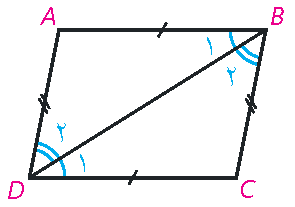
\includegraphics[scale=0.8]{"Shapes/Fasl - 3/Dars 1/qazie 1.pdf"}
	\end{flushleft}
\end{minipage}
%\newline 
%\bigskip \bigskip

{\semibold عکس قضیه ۱}: اگر در یک چهارضلعی، اضلاع مقابل دوبه‌دو هم‌اندازه باشند، چهارضلعی متوازی‌الاضلاع است.

	\begin{minipage}{.75\textwidth}
	فرض: 
	$AB = CD, \; AD = BC$
	\hfill حکم:
	$AB \parallel CD, \; AD \parallel BC$
	\begin{flushleft}
		$ \left. \begin{array}{lll}
			AB = CD \\ AD = BC \\ AC = AC
		\end{array} \right\} \xRightarrow{\mbox{زض‌ز}} \triangle ABC \cong  \triangle ADC 
		\Rightarrow \left. \begin{array}{lll}
			 \widehat{A}_1 = \widehat{C}_1 \Rightarrow AB \parallel CD\\ \widehat{A}_2 = \widehat{C}_2 \Rightarrow AD \parallel BC
		\end{array} \right.$
	\end{flushleft}
\end{minipage}
\begin{minipage}{.25\textwidth}
	\begin{flushleft}
		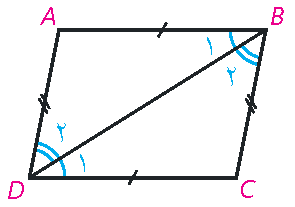
\includegraphics[scale=0.8]{"Shapes/Fasl - 3/Dars 1/qazie 1.pdf"}
	\end{flushleft}
\end{minipage} 

{\semibold قضیه ۲}: در متوازی‌الاضلاع هر دو زاویه‌ی مجاور مکمل‌اند.

\begin{minipage}{.75\textwidth}
	 فرض: 
	$AB \parallel CD, \; AD \parallel BC$
	\hfill حکم:
	$ \left. \begin{array}{rrr}
		\widehat{B}_2 + \widehat{C}_1 = 180^{\circ} \\ \widehat{C}_1 + \widehat{D} = 180^{\circ}
	\end{array} \right\}$
	\begin{flushleft}
		$(AB \parallel CD, \, \text{مورب} \, BC ) \rightarrow \left. \begin{array}{rll}
			  \widehat{C}_1 = \widehat{B}_1 \\ \widehat{B}_1 + \widehat{B}_2 = 180^{\circ} 
		\end{array} \right\} \rightarrow \widehat{C}_1 + \widehat{B}_2 = 180^{\circ} $
	
		$(AD \parallel BC, \, \text{مورب} \, CD ) \rightarrow \left. \begin{array}{rll}
			\widehat{D} = \widehat{C}_2 \\ \widehat{C}_1 + \widehat{C}_2 = 180^{\circ}
		\end{array} \right\} \rightarrow \widehat{D} + \widehat{C}_1 = 180^{\circ}$
	\end{flushleft}
\end{minipage}
\begin{minipage}{.25\textwidth}
	\begin{flushleft}
		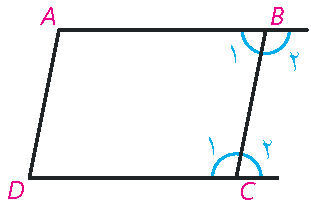
\includegraphics[scale=0.8]{"Shapes/Fasl - 3/Dars 1/qazie 2.pdf"}
	\end{flushleft}
\end{minipage}

{\semibold عکس قضیه ۲}: هر چهارضلعی که ر دو زاویه‌ی مجاور آن مکمل‌ باشند، متوازی‌الاضلاع است.

\begin{minipage}{.75\textwidth}
	 فرض: 
	$\left.
	\begin{array}{rrr}
		B_2 + D =180^{\circ} \\
		C_1 + D =180^{\circ} \\
		A + D = 180^{\circ} \\
		A + B_2 = 180^{\circ}
	\end{array}
	\right\}$
	\hfill حکم:
	$ \left. 
	\begin{array}{rrr}
		AB \parallel CD \\
		AD \parallel BC
	\end{array}
 \right\}$
	\begin{flushleft}
		$ \left.
		\begin{array}{rrr} 
			\widehat{C}_1 + \widehat{C}_2 = 180^{\circ} \\
			\widehat{C}_1 + \widehat{D} = 180^{\circ}
		\end{array}
	 \right\}
	  \rightarrow \widehat{D} = \widehat{C}_2 \Rightarrow AD \parallel BC$
	  
	  $\left.
	  \begin{array}{rrr} 
	  	\widehat{C}_1 + \widehat{B}_2 = 180^{\circ} \\
	  	\widehat{B}_1 + \widehat{B}_2 = 180^{\circ}
	  \end{array}
	  \right\}
	  \rightarrow \widehat{B}_1 = \widehat{C}_1 \Rightarrow AB \parallel CD$
	\end{flushleft}
\end{minipage}
\begin{minipage}{.25\textwidth}
	\begin{flushleft}
		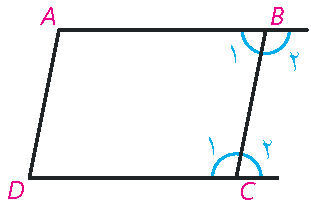
\includegraphics[scale=0.8]{"Shapes/Fasl - 3/Dars 1/qazie 2.pdf"}
	\end{flushleft}
\end{minipage}

{\semibold قضیه ۳}: در هر متوازی‌الضلاع، هر دو زاویه‌ی مقابل هم اندازه‌اند.

\begin{minipage}{.75\textwidth}
	 فرض: 
	$\left.
	\begin{array}{rrr}
		AB \parallel CD \\
		BC \parallel AD
	\end{array}
	\right\}$
	\hfill حکم:
	$ \left. 
	\begin{array}{rrr}
		\widehat{A} = \widehat{C} \\
		\widehat{B} = \widehat{D}
	\end{array}
 \right\}$
 \begin{flushright}
 	 بنا بر قضیه ۲ می‌توان نوشت:
 \end{flushright}
	\begin{flushleft}
		$ \left.
		\begin{array}{rrr} 
			\widehat{A} + \widehat{B} = 180^{\circ} \\
			\widehat{B} + \widehat{C} = 180^{\circ}
		\end{array}
	 \right\}
	 \rightarrow \widehat{A} = \widehat{C}
	 \qquad
	  \left.
	  \begin{array}{rrr} 
	  	\widehat{B} + \widehat{C} = 180^{\circ} \\
	  	\widehat{C} + \widehat{D} = 180^{\circ}
	  \end{array}
	  \right\}
	  \rightarrow \widehat{B} = \widehat{D}$
	\end{flushleft}
\end{minipage}
\begin{minipage}{.25\textwidth}
	\begin{flushleft}
		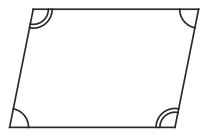
\includegraphics[scale=0.8]{"Shapes/Fasl - 3/Dars 1/qazie 3.pdf"}
	\end{flushleft}
\end{minipage}

{\semibold عکس قضیه ۳}: در هر یک چهارضلعی هر دو زاویه‌ی مقابل هم‌اندازه باشند، چهارضلعی متوازی‌الاضلاع است.

\begin{minipage}{.75\textwidth}
 فرض: 
	$
		\widehat{A} = \widehat{C} = x \; , \; \widehat{B} = \widehat{C} = y
	$
	\hfill حکم:
	$ 
		\mathrm{ABCD}
	$ موازی‌الاضلاع است.
	\begin{flushleft}
		$ 
			x+y +x +y = 360^{\circ} \Rightarrow 2x + 2y = 360^{\circ} \Rightarrow x+y =180^{\circ}
		$
	\end{flushleft}
		هر دو زاویه‌ی مجاور مکمل‌اند،  بنابر عکس قضیه‌ ۲، ABCD متوازی‌الاضلاع است.
\end{minipage}
\begin{minipage}{.25\textwidth}
	\begin{flushleft}
		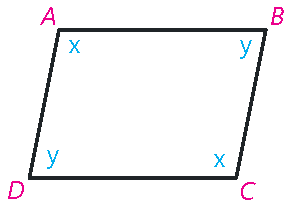
\includegraphics[scale=0.8]{"Shapes/Fasl - 3/Dars 1/qazie 3 ax.pdf"}
	\end{flushleft}
\end{minipage}

{\semibold قضیه ۴}: در هر متوازی‌الاضلاع اقطار منصف یکدیگیرند.

\begin{minipage}{.75\textwidth}
 فرض: 
	$
		AB \parallel CD \; , \; AD = BC
	$
	\hfill حکم:
	$ 
		OA = OC \; , \; OD = OB
	$
	\begin{flushleft}
		$ 
			\left. 
				\begin{array}{crr}
					\widehat{A}_1 = \widehat{C}_1 \\
					\widehat{B}_1 = \widehat{D}_1 \\
					AB = CD
				\end{array}
			\right\}
			\xRightarrow{\mbox{زض‌ز}} \triangle OAB \cong \triangle OCD \Rightarrow \left.
				\begin{array}{lll}
					OA = OC \\
					OB = OD
				\end{array}
			\right.
		$
	\end{flushleft}
\end{minipage}
\begin{minipage}{.25\textwidth}
	\begin{flushleft}
		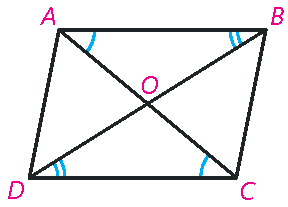
\includegraphics[scale=0.8]{"Shapes/Fasl - 3/Dars 1/qazie 4.pdf"}
	\end{flushleft}
\end{minipage}

{\semibold عکس قضیه ۴}: هر چهارضلعی‌ای که اقطارش منصف یکدیگر باشند، متوازی‌الاضلاع است.\\

\begin{minipage}{.75\textwidth}
 فرض: 
	$
	 OA = OC \; , \; OD = OB
	$
	\hfill حکم:
	$ 
	AB \parallel CD \; , \; AD = BC
	$
	\begin{flushleft}
		$ 
		\left. 
		\begin{array}{crr}
			\widehat{O}_1 = \widehat{O}_2 \\
			OB = OD \\
			OA = OC
		\end{array}
		\right\}
		\xRightarrow{\mbox{ض‌زض}} \triangle OAB \cong \triangle OCD \Rightarrow \left.
		\begin{array}{cll}
			AB = CD \\
			\widehat{A}_1 = \widehat{C}_1 
		\end{array}
		\right.
		$
		$
		\widehat{A}_1 = \widehat{C}_1 \Rightarrow AB \parallel CD,\, \mbox{مورب} AC
		$
		
	\end{flushleft}
\end{minipage}
\begin{minipage}{.25\textwidth}
	\begin{flushleft}
		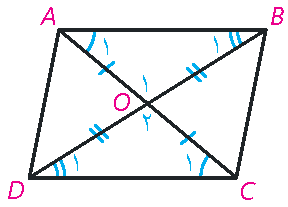
\includegraphics[scale=0.8]{"Shapes/Fasl - 3/Dars 1/qazie 4 ax.pdf"}
	\end{flushleft}
\end{minipage}

هر در چهارضلعی که دو ضلع آن هم‌اندازه و موازی باشند.، متوازی‌الاضلاع است.

\begin{minipage}{.75\textwidth}
فرض: 
	$
	AB = CD \; , \; AB \parallel CD
	$
	\hfill حکم:
	$ 
	BC \parallel AD
	$
	\begin{flushleft}
		$ 
		\left. 
		\begin{array}{crr}
			\widehat{A}_1 = \widehat{C}_1 \\
			AB = CD \\
			AC = AC
		\end{array}
		\right\}
		\xRightarrow{\mbox{ض‌زض}} \triangle ABC \cong \triangle ACD \Rightarrow
		\widehat{A}_2 = \widehat{C}_2 
		$
		$
		\widehat{A}_2 = \widehat{C}_2 \Rightarrow AD \parallel BC,\, \mbox{مورب} AC
		$
		
	\end{flushleft}
\end{minipage}
\begin{minipage}{.25\textwidth}
	\begin{flushleft}
		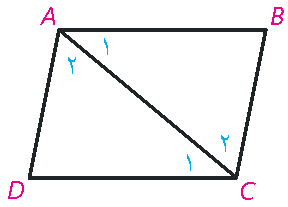
\includegraphics[scale=0.8]{"Shapes/Fasl - 3/Dars 1/2-1.pdf"}
	\end{flushleft}
\end{minipage}

\subsection{ویژگی‌هایی از مستطیل و لوزی}
در مستطیل 
$
ABCD
$،
دو قطر را رسم می‌کنیم. از هم‌نهشتی دو مثلث 
$
ACD
$
و
$
BCD
$
می‌توان نتیجه گرفت \\
$
AC = BD
$.

\begin{minipage}{.75\textwidth}
	\begin{flushleft}
		$ 
		\left. 
		\begin{array}{crr}
			\widehat{D} = \widehat{C} \\
			AD = BC \\
			CD = CD
		\end{array}
		\right\}
		\xRightarrow{\mbox{ض‌زض}} \triangle ACD \cong \triangle BCD \Rightarrow
		AC = BD
		$
		
	\end{flushleft}
\end{minipage}
\begin{minipage}{.25\textwidth}
	\begin{flushleft}
		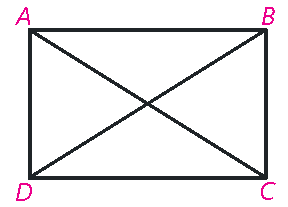
\includegraphics[scale=0.8]{"Shapes/Fasl - 3/Dars 1/2-1.1.pdf"}
	\end{flushleft}
\end{minipage}

بنابراین در هر مستطیل اقطار برابرند.

اگر دو قطر یک چهار ضلعی هم‌اندازه باشند. نمی‌توان نتیجه گرفت که آن چهارضلعی مستطیل است، ولی اگر آن چهارضلعی متوازی‌الاضلاع باشد، حتما مستطیل است.

\begin{minipage}{.65\textwidth}
	\begin{flushleft}
		$ 
		\left. 
		\begin{array}{crr}
			AC = BD \\
			AD = BC \\
			CD = CD
		\end{array}
		\right\}
		\xRightarrow{\mbox{ض‌ض‌ض}} \triangle ACD \cong \triangle BCD 
		\rightarrow 
		\widehat{D} =\widehat{C} = 90^{\circ}
		$
		
	\end{flushleft}
\end{minipage}
\begin{minipage}{.39\textwidth}
	\begin{flushleft}
		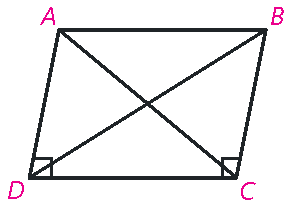
\includegraphics[scale=0.8]{"Shapes/Fasl - 3/Dars 1/2-1.3.pdf"}
		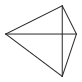
\includegraphics[scale=0.8]{"Shapes/Fasl - 3/Dars 1/2-1.2.pdf"}
	\end{flushleft}
\end{minipage}

\subsection{ویژگی‌ مهمی در مثلث قائم‌الزاویه}
در هر مثلث قائم‌الزاویه ‌اندازه‌ی میانه‌ی وارد بر وتر نصف اندازه‌ی وتر است.
 
 \begin{minipage}{.75\textwidth}
 	 فرض: 
 	$
 	\widehat{A} = 90^{\circ} \; , \; BM = MC
 	$
 	\hfill حکم:
 	$ 
 	AM = \dfrac{BC}{2}
 	$
 	\newline
 	
 	روی نیم‌خط $AM$ نقطه‌ی $D$ را چنان در نظر می‌گیریم که $DM = AM$.
 	\begin{flushleft}
 		$ 
	 		\left. 
		 		\begin{array}{crr}
		 			BM = CM \\
		 			AM = DM 
		 		\end{array}
	 		\right\}
	 		\Rightarrow \mbox{متوازی‌الاضلاع } ABCD \xRightarrow{\widehat{A} = 90^{\circ}} \mbox{مستطیل } ABCD
 		$

		$
			\Rightarrow AD = BC \Rightarrow
			BM = CM = AM = DM \Rightarrow AM = \dfrac{BC}{2}
		$

 	\end{flushleft}
 \end{minipage}
 \begin{minipage}{.25\textwidth}
 	\begin{flushleft}
 		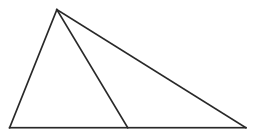
\includegraphics[scale=0.8]{"Shapes/Fasl - 3/Dars 1/2-2.1.pdf"}
 	\end{flushleft}
 \end{minipage}
 
 اگر در مثلثی اندازه‌ی میانه‌ی وارد بر ضلع، نصف اندازه‌ی آن ضلع باشد، آن مثلث قائم‌الزاویه‌ است.
 
  \begin{minipage}{.7\textwidth}
 	 فرض: 
 	$
 	 AM = \dfrac{BC}{2} \; , \; BM = CM
 	$
 	\hfill حکم:
 	$ 
 	\widehat{A} = 90^{\circ}
 	$\\
 	روی نیم‌خط $AM$ نقطه‌ی $D$ را چنان در نظر می‌گیریم که $DM = AM$.
 	\begin{flushleft}
 		$ 
	 		\left. 
		 		\begin{array}{crr}
		 			AM = \dfrac{BC}{2} \\
		 			\dfrac{AD}{2} = AM = DM
		 		\end{array}
	 		\right\}
	 		\Rightarrow \dfrac{BC}{2} = \dfrac{AD}{2} \Rightarrow BC =AM 
 		$
 		$
			\left. 
	 			\begin{array}{crr}
	 				\dfrac{AD}{2} =  AM = DM\\
	 				\dfrac{BC}{2} = BM = CM
	 			\end{array}
			\right\}
 			\Rightarrow AM = BM = CM = DM
 		$
 		$
 			\Rightarrow \mbox{مستطیل‌} ANCD \Rightarrow \widehat{A} = 90^{\circ}
 		$
 		
 	\end{flushleft}
 \end{minipage}
 \begin{minipage}{.3\textwidth}
 	\begin{flushleft}
 		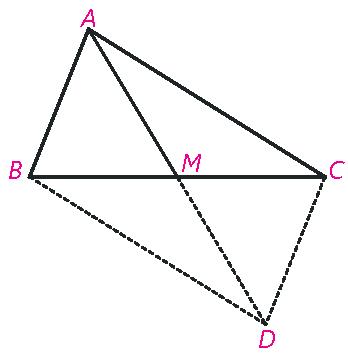
\includegraphics[scale=0.8]{"Shapes/Fasl - 3/Dars 1/2-2.2.pdf"}
 	\end{flushleft}
 \end{minipage}
 

\subsection{ویژگی‌هایی که فقط در لوزی برقرارند}

\begin{minipage}{.8\textwidth}
	
	اقطار لوزی
	$ABCD$
	را رسم می‌کنیم. چون لوزی متوازی‌الاضلاع است، اقطار منصف یکدیگرند. 
	$
	\triangle ABD
	$
	نیز متساوی‌الساقین است.
	
	نقطه تلاقی دو قطر را
	$H$
	می‌نامیم، در مثلث
	$ABD$،
	$AH$
	عمودمنصف
	$BD$
	و روی نیمساز 
	$
	\widehat{A}
	$
	است.
	
	بنابراین؛

 در هر لوزی اقطار {\medium عمودمنصف} یکدیگیر و روی {\medium نیمساز} زوایا هستند.

\end{minipage}
\begin{minipage}{.2\textwidth}
	\begin{flushleft}
		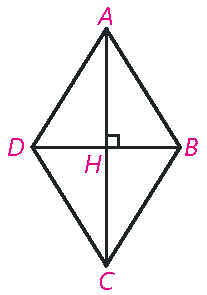
\includegraphics[width=3cm]{"Shapes/Fasl - 3/Dars 1/2-3.1.pdf"}
	\end{flushleft}
\end{minipage}

\subsection{ذوزنقه}
ذوزنقه چهارضلعی‌ای است که با چهارضلعی‌هایی که قبلاً بررسی کردیم، کمی متفاوت است.

{\semibold تعریف:} ذوزنقه چهارضلعی‌ای است که فقط دو ضلع آن موازی باشند.

\begin{minipage}{.67\textwidth}

هر یک از دو ضلع $AB$، $CD$ را که موازی‌اند،
 {\medium قاعده} و هر یک از دو ضلع غیر موازی را {\medium ساق} می نامند. از موازی بودن قاعده‌های $AB$ ، $CD$ و قاطع‌های $BC$ و $AD$ در زوایا می‌توان نتیجه گرفت که:
\newline

زوایای $ \widehat{A}$ و $ \widehat{ِD}$ مکمل‌اند، همچنین زوایای  $ \widehat{B}$ و $ \widehat{C}$ مکمل هستند.
\newline

اگر در یک ذوزنقه یک ساق برابر باشند، آن را ذوزنقه متساوی‌الساقین می‌نامند.
\newline

هرگاه در یک ذوزنقه یک ساق بر قاعده‌ها عمود باشد، مسلماً بر قاعده‌ی دیگر نیز عمود است. در این صورت ذوزنقه را قائم‌الزاویه می‌نامند.
\end{minipage}
\begin{minipage}{.3\textwidth}
	\begin{flushleft}
		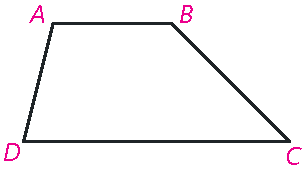
\includegraphics{"Shapes/Fasl - 3/Dars 1/2-4.1.pdf"}
		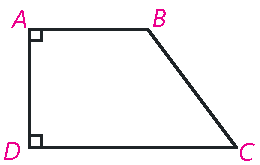
\includegraphics{"Shapes/Fasl - 3/Dars 1/2-4.2.pdf"}
	\end{flushleft}
\end{minipage}

در هر ذوزنقه‌ی متساوی‌الساقین زاویه‌های مجاور به یک قاعده هم‌اندازه‌اند.

\begin{minipage}{.7\textwidth}

	فرض:
	$
		\left.
			\begin{array}{ccc}
				AD = BC \\
				AB \parallel CD
			\end{array}
		\right\}
	$
	\hfill
	حکم:
	$
		\left.
			\begin{array}{ccc}
				\widehat{C} = \widehat{D} \\
				\widehat{A} = \widehat{B}
			\end{array}
		\right\}
	$

\begin{flushleft}
	$
	\left.
	\begin{array}{ccc}
		AD = BF \\
		AD = BC
	\end{array}
	\right\}
	\Rightarrow BF = BC  \rightarrow \widehat{E}_1 = \widehat{C}
	$
	
	$
	\left.
	\begin{array}{ccc}
		\widehat{E}_1 = \widehat{C} \\
		\widehat{E}_1 = \widehat{D}
	\end{array}
	\right\}
	\Rightarrow \widehat{C} = \widehat{D}
	$
\end{flushleft}
\end{minipage}
\begin{minipage}{.3\textwidth}
\begin{flushleft}
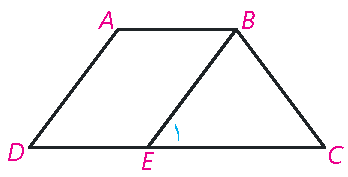
\includegraphics[scale=0.8]{"Shapes/Fasl - 3/Dars 1/2-4.3.pdf"}
\end{flushleft}
\end{minipage}

اگر در یک ذوزنقه دو زاویه‌ی مجاور به یک قاعده هم‌اندازه باشند، ذوزنقه متساوی‌الساقین است.

\begin{minipage}{.7\textwidth}
		فرض:
		$
		\left.
		\begin{array}{ccc}
			\widehat{C} = \widehat{D} \\
			AB \parallel CD
		\end{array}
		\right\}
		$
		\hfill
		حکم:
		$
		\left.
		\begin{array}{ccc}
			 AD = BC 
		\end{array}
		\right\}
		$

	\begin{flushleft}
		$
		\left.
		\begin{array}{ccc}
			\widehat{D} = \widehat{E}_1 \\
			\widehat{C} = \widehat{D}
		\end{array}
		\right\}
		\Rightarrow \widehat{E}_1 = \widehat{C} \rightarrow  BE = BC 
		$
		
		$
		\left.
		\begin{array}{ccc}
			 BF = BC  \\
			AD = BF
		\end{array}
		\right\}
		\Rightarrow AD = BC
		$
	\end{flushleft}
\end{minipage}
\begin{minipage}{.3\textwidth}
	\begin{flushleft}
		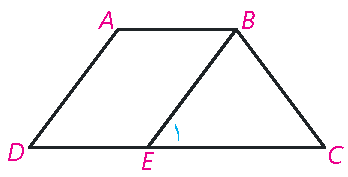
\includegraphics[scale=0.8]{"Shapes/Fasl - 3/Dars 1/2-4.3.pdf"}
	\end{flushleft}
\end{minipage}

در هر ذوزنقه‌ی متساوی‌الساقین، اقطار اندازه‌های مساوی دارند و برعکس.
\smallskip

\begin{minipage}{.7\textwidth}
		فرض:
		$
		AB \parallel CD , AD = BC
		$
		\hfill
		حکم:
		$
		AC = BD
		$
	\begin{flushleft}
		$
		\left.
		\begin{array}{ccc}
			AD = BC \\
			CD = CD \\
			\widehat{C} = \widehat{D}
		\end{array}
		\right\}
		\xRightarrow{\mbox{ض‌زض}} \triangle BDC \equiv \triangle ADC \rightarrow  AC = BD 
		$
	\end{flushleft}
\end{minipage}
\begin{minipage}{.3\textwidth}
	\begin{flushleft}
		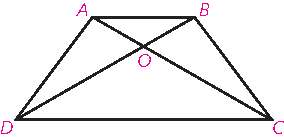
\includegraphics{"Shapes/Fasl - 3/Dars 1/PDFs/P63-S1.pdf"}
	\end{flushleft}
\end{minipage}

\begin{minipage}{.7\textwidth}
		
		فرض:
		$
		AC = BD
		$
		\hfill
		حکم:
		$
		AD = BC
		$
	\begin{flushleft}
		$
		\left.
		\begin{array}{ccc}
			AH' = BH \\
			AC = BD 
		\end{array}
		\right\}
		\xRightarrow{\mbox{وض}} \triangle AH'C \cong \triangle BHD \rightarrow  D_1 = C_1 
		$
		\smallskip
		
		$
		\left.
		\begin{array}{ccc}
			D_1 = C_1 \\
			CD = CD  \\
			AC = BD
		\end{array}
		\right\}
		\xRightarrow{\mbox{ض‌زض}} \triangle ADC \cong \triangle ‌BDC \rightarrow  AD = BC
		$
	\end{flushleft}
\end{minipage}
\begin{minipage}{.3\textwidth}
	\begin{flushleft}
		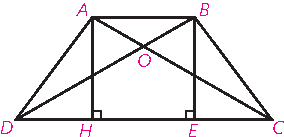
\includegraphics{"Shapes/Fasl - 3/Dars 1/PDFs/P63-S2.pdf"}
	\end{flushleft}
\end{minipage}
\newpage

%\textbf{تمرین}
\subsection{تمرین}
	\begin{multicols}{2}
			{\medium ۱-} در کدام n ضلعی تعداد اقطار و اضلاع برابر است؟
			\bigskip
			
				{\medium ۲- }در دو چهارضلعی مقابل 
			$ AB = A'B' $
			و
			$ \angle B = \angle B' $
			و
			$ BC = B'C' $
			و
			$ \angle C = \angle C' $
			و
			$ CD = C'D' $
			است. چگونه مساوی بودن اندازه‌های سایر ضلع‌ها و زاویه‌ها را نتیجه می‌گیرید؟
			
			اگر 
			$ \angle B = \angle B' $
			و
			$ BC = B'C' $
			و
			$ \angle C = \angle C' $
			و
			$ CD = C'D' $
			و
			$ \angle D = \angle D' $
			در این حالت چگونه مساوی بودن اندازه‌های سایر ضلع‌ها و زاویه‌ها را نتیجه می‌گیرید؟

		\begin{Figure}
			\centering
			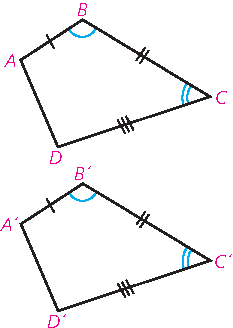
\includegraphics[scale=1.2]{"Shapes/Fasl - 3/Dars 1/PDFs/P63-S3,4.pdf"}
			\captionof{figure}{تمرین ۲}
		\end{Figure}

\bigskip
				{\medium ۳-} از تقاطع نیم‌سازهای داخلی یک متوازی‌الضلاع، چهارضلعی
			MNPQ
			پدید آمده‌است. ثابت کنید این چهارضعلی مستطیل است.
			




		\begin{Figure}
			\centering
			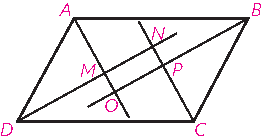
\includegraphics[scale=1.2]{"Shapes/Fasl - 3/Dars 1/PDFs/P63-S5.pdf"}
			\captionof{figure}{تمرین ۳}
		\end{Figure}

			\bigskip
			{\medium ۴-}مثلث قائم الزاویه‌ی 
			$\triangle ABC$
			را که در آن 
			$\angle A$
			قائمه و اندازه‌ی
			$\angle C$
			برابر 
			$30^{\circ}$
			است، در نظر می‌گیریم. میانه‌ی وارد بر وتر را رسم کنید. مثلث های 
			$AMC$
			و
			$AMB$
			چگونه مثلث‌هایی هستند؟ نشان دهید 
			$AB = \dfrac{BC}{2}$
			یعنی در هر مثلث قائم الزاویه اگر اندازه‌ی یک زاویه 
			$30^{\circ}$
			باشد، اندازه‌ی ضلع مقابل آن نصف اندازه‌ی وتر است.
			
			سپس با استفاده از قضیه‌ی فیثاغورث نشان دهید: 
			$AC = \frac{\sqrt{3}}{2}BC$.
			
			یعنی در هر مثلث قائم الزاویه اگر یک زاویه 
			$60^{\circ}$
			باشد، اندازه‌ی ضلع مقابل آن  اندازه‌ی وتر است.
			
			اکنون مثلث قائم الزاویه ای رسم کنید که اندازه‌ی یک زاویه‌ی آن 
			$45^{\circ}$
			باشد و نشان دهید که اندازه‌ی هر ضلع زاویه‌ی قائمه در آن 
			$\frac{\sqrt{2}}{2}$
			اندازه‌ی وتر است.

		\begin{Figure}
			\centering
			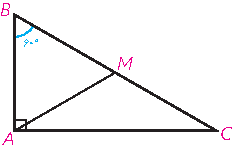
\includegraphics[scale=1.2]{"Shapes/Fasl - 3/Dars 1/PDFs/P64-S1.pdf"}
			\captionof{figure}{تمرین ۴}
		\end{Figure}

			\bigskip
			{\medium ۵-}در مثلث قائم الزاویه‌ی 
			$\triangle ABC$
			اندازه‌ی زاویه‌ی 
			$\widehat{B}$
			برابر 
			$15^{\circ}$
			است. با رسم میانه و ارتفاع وارد بر وتر نشان دهید اندازه‌ ارتفاع وارد بر وتر 
			$\frac14$
			اندازه‌ی وتر است.
			
			\begin{Figure}
				\centering
				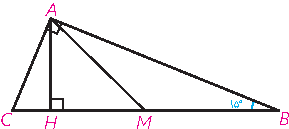
\includegraphics[scale=1.2]{"Shapes/Fasl - 3/Dars 1/PDFs/P64-S2.pdf"}
				\captionof{figure}{تمرین ۵}
			\end{Figure}


		
			\bigskip
			 {\medium ۶-} در متوازی الاضلاع  
			$ABCD$،
			$M$ و $N$
			به ترتیب وسط های ضلع های 
			$AD$ و $BC$
			می‌باشند. چرا خطوط
			$MB$ و $ND$
			موازی‌اند؟ \\
			به کمک آن ثابت کنید: $AP = PQ = QC$.
	
\begin{Figure}
	\centering
	\includegraphics[scale=1.2]{"Shapes/Fasl - 3/Dars 1/PDFs/P64-S3"}
	\captionof{figure}{تمرین ۶}
	\label{fig:p64-s3}
\end{Figure}


			\bigskip
			{\medium 7-}ثابت کنید اگر وسط های ضلع‌های هر چهارضلعی را به طور متوالی به هم وصل کنیم، یک متوازی‌الاضلاع پدید می‌آید.
			
			این چهارضلعی باید چه ویژگی‌ای داشته‌ باشد تا این متوازی‌الاضلاع مستطیل یا لوزی شود؟
			
			چه رابطه‌ای بین محیط متوازی‌الاضلاع پدید آمده با اندازه‌های قطر‌های چهارضلعی اولیه وجود دارد؟
			
			\bigskip
			{\medium 8-} 
			تعداد اقطار یک چند ضلعی محدب از تعداد اضلاع آن ۴۲ تا بیشتر است. این چند ضلعی چند قطر دارد؟
			
			\bigskip
			{\medium 9-} 
			مجموع تعداد اضلاع و اقطار یک 1 $\!+\!$ n ضلعی نصف اقطار یک 2n ضلعی است.  n چند است؟
			
			\bigskip
			{\medium 10-} 
			در یک ۱۰۰ ضلعی محدب تعداد اقطاری که از ۲ رأس غیرمجاور می‌گذرد چند تا است؟
			
			\bigskip
			{\medium 11-} 
			مجموع تعداد اقطار و اضلاع یک چند ضلعی محدب برابر ۱۲۰ است. تعداد اضلاع چند است؟
			
			\bigskip
			{\medium 12-}
			تعداد اقطار یک چند ضلعی ۳۵ است. از هر رأس این چندضلعی چند قطر می‌گذرد؟
	\end{multicols}


\newpage

\subsection{پاسخ}
	\subsubsection[1]{۱)}
	\begin{flushleft}
		$
			n = \dfrac{n(n-3)}{2} \Rightarrow 2n = n^2 - 3n \Rightarrow n^2 -5n = 0 \Rightarrow n(n-5) = 0 \Rightarrow 
			\left\{
				\begin{array}{lll}
					x = 0 & \mbox{ق‌ق} \\
					\fbox{$x = 5$} &  \mbox{غ‌ق‌ق} 
				\end{array}
			\right.
		$
	\end{flushleft}
	\subsubsection[2]{۲)}
	\bigskip \bigskip \bigskip
	  
	\subsubsection[3]{۳)}   
   	\begin{flushleft}
	$
   		\left.
   			\begin{array}{lll}
   				\widehat{B} = \widehat{C} = 180^{\circ} \Rightarrow 2 \alpha + 2 \beta =180^{\circ} \Rightarrow \alpha + \beta = 90^{\circ}  \Rightarrow \widehat{P}_1 = \widehat{P}_2 = 90^{\circ} \\
			   	\widehat{A} = \widehat{D} = 180^{\circ} \Rightarrow 2m + 2n =180^{\circ} \Rightarrow m + n = 90^{\circ}  \Rightarrow \widehat{M}_2 = \widehat{M}_1 = 90^{\circ} \\
			   	\widehat{C} = \widehat{D} = 180^{\circ} \Rightarrow 2 n + 2 \alpha =180^{\circ} \Rightarrow m + \alpha = 90^{\circ}  \Rightarrow \widehat{N}_1 = \widehat{N}_2 = 90^{\circ}  \\
	   	   		\widehat{P}_2 + \widehat{M}_1 + \widehat{N}_2 + \widehat{Q}_2= 360^{\circ} \Rightarrow 270^{\circ} + \widehat{Q}_2 = 360^{\circ} \Rightarrow \widehat{Q}_2 = 90^{\circ} 
   			\end{array}
   		\right\}
   		\Rightarrow \mbox{\lr{MNPQ} مستطیل}
   	$
   \end{flushleft}
   
	\subsubsection[4]{۴)}

			\begin{flushleft}
					$
					BM = AM \Rightarrow \text{\lr{ABM} متساوی‌الاضلاع است}
				$,
				$
					CM = AM \Rightarrow \text{\lr{ACM} متساوی‌الساقین است}
				$
				$
					AB = \dfrac{BC}{2} \Rightarrow AB =MB = \dfrac{BC}{2}
				$
				
				$
					AB^2 + AC^2 = BC^2 \Rightarrow \dfrac{BC^2}{4} + AC^2 = BC^2 \Rightarrow AC^2 = BC^2 - \dfrac{BC^2}{4} \Rightarrow AC^2 = 3bc^2 \Rightarrow AC = BC \dfrac{\sqrt{3}}{2}
				$
			\end{flushleft}

	\subsubsection[5]{۵)}
	
	     	\begin{flushleft}
	     		$ \triangle AHM:$
	     		$
	     			\left.
		     			\begin{array}{lcc}
		     			    &	\widehat{M} = \left. 30^{\circ} \right\} \rightarrow & AH = \frac12 AM \\
		     				& &AM = \frac12 BC
		     			\end{array}
	     			\right\}
	     			\rightarrow AH = \frac12 \left( \frac12 BC \right) \Rightarrow AH = \frac14 BC
	     		$
	     	\end{flushleft}


	\subsubsection[6]{۶)}
	\bigskip \bigskip \bigskip
	
	\subsubsection[7]{۷)}
	\bigskip \bigskip \bigskip
	
	\subsubsection[8]{8)}
	\begin{flushleft}
		$\dfrac{n(n-3)}{2} = x+42 \Rightarrow x^2 -3x = 2x +84 \Rightarrow x^2 -5x -84 =0 \Rightarrow (x+7)(x-12) = 0  \Rightarrow \left\{ \begin{array}{lll}
			\fbox{$x = 12$} & \mbox{ق‌ق} \\ x = -7 & \mbox{غ‌ق‌ق}
		\end{array} \right.$
	\end{flushleft}
	
	\subsubsection[9]{9)}
	\begin{flushleft}
		$\dfrac{n+1(n+1-3)}{2} + n+1 = \dfrac{2n(2n-3)}{4} \Rightarrow \dfrac{n^2-n-2}{2}+ n+1 = \dfrac{4n^2-6n}{4} \Rightarrow \dfrac{n^2-n-2+2n+2}{2} = \dfrac{2n^2-3n}{2} \Rightarrow n^2+n = 2n^2 -3n \Rightarrow n^2 -4n = 0 \Rightarrow n(n-4) = 0  \Rightarrow \left\{ \begin{array}{lll}
			n =0 & \mbox{غ‌ق‌ق} \\ \fbox{$n = 4$} & \mbox{ق‌ق}
		\end{array} \right.$
	\end{flushleft}

	\subsubsection[10]{10)}
	\begin{flushleft}
		$100 - 3 = 97 \qquad (2 \times 97) - 1 = 193$
	\end{flushleft}
	
	
	\subsubsection[11]{11)}
	\begin{flushleft}
		$\dfrac{n+1(n+1-3)}{2} + n = 120 \Rightarrow \dfrac{2n^2-3}{2} = 120 \Rightarrow n^2-n=240 \Rightarrow (n-16)(n+15) = 0 \Rightarrow \left\{ \begin{array}{lll}
			\fbox{$n = 16$} & \mbox{ق‌ق} \\ n =-17 & \mbox{غ‌ق‌ق}
		\end{array} \right.$
	\end{flushleft}

	\subsubsection[12]{12)}
	\begin{flushleft}
		$\dfrac{n(n-3)}{2} = 35 \Rightarrow x^2 -3x = 70 \Rightarrow (x-10)(x+7) = 0 \Rightarrow \left\{ \begin{array}{lll}
		\fbox{$x =10$} & \mbox{ق‌ق} \\ x = -7 & \mbox{غ‌ق‌ق}
	\end{array} \right.$
	\end{flushleft}

\newpage
\section{مساحت و کاربردهای آن}

\textbf{یادآوری}

\begin{minipage}{0.7\textwidth}
	١- اگر اندازهٔ یک ضلع مربع $a$ باشد، $S=a^2$ مساحت آن است.
	
	۲- اگر اندازهٔ یک ضلع مثلث $a$ و اندازهٔ ارتفاع نظیر آن ضلع $h_a$ باشد، آنگاه 
	$S=\frac12 ah_a$
	
	بنابراین در هر مثلث ABC اگر اندازه‌ی اضلاع ،BC AC و AB را به ترتیب با ،a b و c اندازه‌های ارتفاع‌های نظیر آن‌ها را به ترتیب با $h_a$، $h_b$ و $h_c$ نشان دهیم آن‌گاه، \\
 $2S = ah_a = bh_b = ch_c$.
	\end{minipage}
\begin{minipage}{0.3\textwidth}
\begin{flushleft}
		\includegraphics{"Shapes/Fasl - 3/Dars 2/P65-S1"}
\end{flushleft}
\end{minipage}

\begin{minipage}{0.7\textwidth}
۳- اگر اندازهٔ یک ضلع متوازی الاضلاع a و اندازهٔ ارتفاع نظیر آن h باشد، 
 $S=ah$.

۴-اگر اندازه های دو قطر لوزی m و n باشند، $S=\frac12 nm$.
	
۵- اگر اندازه های دو قاعدهٔ یک ذوزنقه a و b و اندازه‌ی ارتفاع آن h باشد\\
	 $S = \dfrac{(a+b)h}2$
\end{minipage}
\begin{minipage}{0.3\textwidth}
	\begin{flushleft}
		\includegraphics{"Shapes/Fasl - 3/Dars 2/P65-S2"}
	\end{flushleft}
\end{minipage}

\bigskip

\textbf{کار در کلاس}

\begin{minipage}{0.7\textwidth}
	فرض کنیم اندازهٔ هر ضلع مثلث متساوی الاضلاع ABC برابر a باشد، ارتفاع AH را رسم کنید. ارتفاع AH میانه نیز است؛ چرا؟
	\begin{flushleft}
		$
	\left.
	\begin{array}{ccc}
		AB = AC \\
		\angle C = \angle B
	\end{array}
	\right\}
	\xrightarrow{\mbox{وز}} \triangle ABH \cong \triangle ACH \Rightarrow CH = BH
	$
	\end{flushleft}
	به کمک قضیهٔ فیثاغورس نشان دهید 
	$AH = \dfrac{a\sqrt{3}}2$
	و 
	$S = \dfrac{a^2 \sqrt{3}}{4}$.
\end{minipage}
\begin{minipage}{0.25\textwidth}
	\begin{flushleft}
		\includegraphics{"Shapes/Fasl - 3/Dars 2/P65-S3"}
	\end{flushleft}
\end{minipage}

	\begin{flushleft}
	$
	AC^2 = AH^2 + CH^2 \Rightarrow a^2 = AH^2 + \dfrac{a^2}{4} \Rightarrow AH^2 = a^2 - \cfrac{a^2}{4} \Rightarrow AH^2 = \dfrac{a^2}{4} \Rightarrow AH = \dfrac{a\sqrt{3}}{2}
	$
	
	$
	\mathrm{S} = \dfrac12 \times a \times \dfrac{a\sqrt{3}}{2} = \dfrac{a^2\sqrt{3}}{4}
	$
\end{flushleft}


\bigskip

\textbf{فعالیت}

\begin{minipage}{0.65\textwidth}
	در چهارضلعی ABCD دو قطر AC و DB برهم عموداند.
	\begin{flushleft}
		$ S_{ADB} = BD \times AH \times \frac12 \hfill S_{DBC} = BD \times CH \times \frac12 $
	\end{flushleft}
	با جمع این دو مساحت داریم:
	\begin{flushleft}
		$S_{ABCD} = \frac12 BD (AH + BH) = \frac12 BD \times AC$
	\end{flushleft}
\end{minipage}
\begin{minipage}{0.3\textwidth}
	\begin{flushleft}
		\includegraphics{"Shapes/Fasl - 3/Dars 2/P65-S4"}
	\end{flushleft}
\end{minipage}

بنابراین؛

در هر چهارضلعی‌ای که دو قطر آن برهم عمود باشند، مساحت برابر است با نصف حاصل ضرب دو قطر.

\subsection{کاربردهایی از مساحت}

قبلاً با کاربرد مساحت در اثبات قضیهٔ تالس آشنا شدید. بعضی رابطه ها و ویژگی‌هایی را که با آن آشنا شده اید یادآوری می‌کنیم.
\bigskip

{\semibold ویژگی ۱}:
در دو مثلث اگر اندازه‌ی قاعده‌ها برابر باشند، نسبت مساحت‌ها برابر نسبت اندازه‌ی ارتفاع‌های متناظر این قاعده‌هاست. \hfill
		$
			\dfrac{S}{S'} = \dfrac{h}{h'}
		$



 \bigskip

{\semibold ویژگی ۲}:
 برابر نسبت اندازه‌های قاعده‌های متناظر این دو ارتفاع است.
 \bigskip
 
 \textbf{کار در کلاس}
 
 \begin{minipage}{0.65\textwidth}
 	نشان دهید یک میانه در هر مثلث، آن را به دو مثلث با مساحت‌های برابر تقسیم می‌کند.
 	\begin{flushleft}
 		$\left.
 		\begin{array}{ccc}
 			S_{ABM} = \frac12 \times h \times BM \\
 			S_{ACM} = \frac12 \times h \times CM
 		\end{array}
 		\right\}
 		\xrightarrow{BM = CM} S_{ABM} = S_{ACM}
 		$
 	\end{flushleft}
 \end{minipage}
 \begin{minipage}{0.3\textwidth}
 	\begin{flushleft}
 		\includegraphics{"Shapes/Fasl - 3/Dars 2/P66-S1"}
 	\end{flushleft}
 \end{minipage}

اگر $\mathrm{F}$ هر نقطه‌ای روی میانه‌ی $\mathrm{AM}$ به جز نقطه‌ی $\mathrm{AM}$ باشد آیا $\mathrm{S_{FBM} = F_{FMC}}$ است؟ چرا؟

\textit{بله؛ 
	$\mathrm{FM}$
	میانه‌ی مثلث 
	$\mathrm{FBC}$
	است پس آن را به دو مثلث هم مساحت تقسیم می‌کند.}

%\textbf{فعالیت}

\newpage


\subsection{نقاط شبکه‌ای و مساحت}

	  \begin{minipage}{0.7\textwidth}
در دو مثلث که اندازه‌ی دو ارتفاع برابر باشد، نسبت مساحت‌ها نقاط شبکه ای و مساحت مطابق شکل نقطه ها روی خط های افقی و عمودی واقع اند؛ به طوری که فاصلهٔ هر دو نقطه متوالی روی یک خط افقی (عمودی)برابر واحد است. چنین نقاطی را نقاط شبکه ای و چندضلعی‌هایی مانند
\lr{ABCD}
را که تمام رأس های آنها روی نقاط شبکه ای واقع اند، چندضلعی های شبکه ای می نامند.
\end{minipage}   
\begin{minipage}{.3\textwidth}
	\begin{flushleft}
		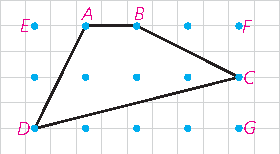
\includegraphics{"Shapes/Fasl - 3/Dars 2/P69-S1.pdf"}
	\end{flushleft}
\end{minipage}

نقاط شبکه ای روی رأس ها و ضلع های چندضلعی را نقاط مرزی و نقاط شبکه ای درون چندضلعی ها را نقاط درونی شبکه ای برای چندضلعی شبکه ای می نامند.

به طور مثال در شکل بالا چهارضلعی 
\lr{ABCD}
یک چهارضلعی شبکه ای است که دارای ۴ نقطهٔ مرزی و ٣ نقطه درونی شبکه ای است.
\bigskip

در چندضلعی های شبکه ای، تعداد نقاط مرزی شبکه ای را با
\lr{b}
و تعداد نقاط درونی شبکه ای را با
\lr{i}
نشان می دهند. اکنون می خواهیم به طور شهودی رابطه ای بین مساحت چندضلعی شبکه ای و نقاط مرزی و درونی شبکه ای نظیر آن را پیدا کنیم.
\bigskip

\textbf{فعالیت}

۱ـ یک چندضلعی شبکه ای حداقل چند نقطهٔ مرزی می تواند داشته باشد؟ چرا؟ \\
حداقل ۳ تا؛ زیرا برای رسم مثلث شبکه‌ای حداقل به ۳ نقطه نیازمندیم.




\begin{minipage}{0.68\textwidth}
	۲ـ یک چندضلعی شبکه ای حداقل چند نقطهٔ درونی می تواند داشته باشد؟ \\
	 صفر
	
	۳ـ در تمام چندضلعی های شبکه ای زیر تعداد نقطه های درونی شبکه ای صفر است، یعنی
	0\lr{i=}
	و تعداد نقاط مرزی، 
	$\mbox{b} = 3 , 4, 5, 6 , 7$
\end{minipage}   
\begin{minipage}{.32\textwidth}
	\begin{flushleft}
		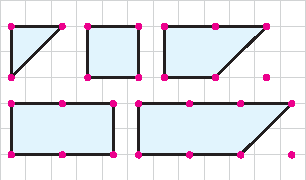
\includegraphics{"Shapes/Fasl - 3/Dars 2/P70-S1.pdf"}
	\end{flushleft}
\end{minipage}

فرمول مساحت اشکال شبکه‌ای به این صورت است: 
$S = \dfrac{b}{2} -1 + i$

توجه داشته باشید که این فرمول را به طور شهودی پیدا کرده ایم. اثبات دقیق این فرمول در حالت کلی نیاز به مقدمات بیشتری دارد.

این فرمول به فرمول {\medium پیک} معروف است که جرج الکساندر پیک (۱۸۵۹-۱۹۴۳) آن را کشف کرد و از سال ۱۹۷۰ به طور گسترده‌ای در کتاب‌های هندسهٔ مقدماتی به کار برده شده است.

به کمک این فرمول می توانیم مساحت شکل های نامنظم هندسی را نیز به طور تقریبی پیدا کنیم.

چندضلعی های 
\lr{A} ،
\lr{B} ،
\lr{C} و
\lr{D}
را در شکل های زیر درنظر بگیرید. ابتدا به روش های هندسی که از قبل می دانید، مساحت آنها را محاسبه کنید؛ سپس با تعیین تعداد نقاط مرزی و درونی، جدول زیر را تکمیل و فرمول پیک را در آنها تحقیق کنید.
\smallskip

\begin{minipage}{1\textwidth}
	\begin{center}
		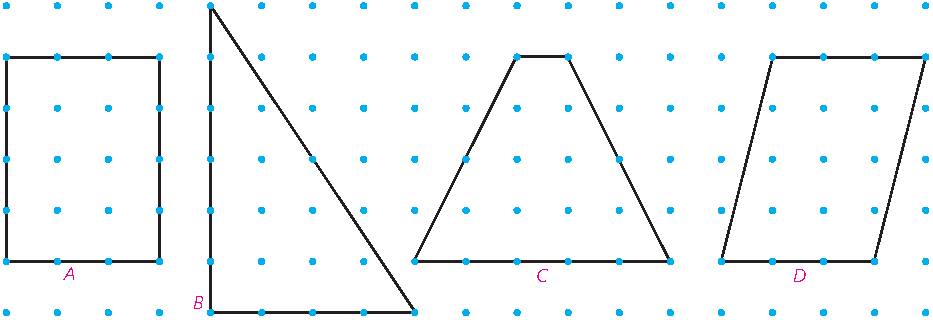
\includegraphics{"Shapes/Fasl - 3/Dars 2/P71-S1.pdf"}
	\end{center}
\end{minipage}

\newpage

\subsection{تمرین}
\begin{multicols}{2}


{\medium ۱- }در یک لوزی اندازهٔ هر ضلع 
$2\sqrt{10}$
و نسبت اندازه های دو قطر
$\dfrac12$
است. مساحت لوزی را پیدا کنید.

\begin{Figure}
	\centering
	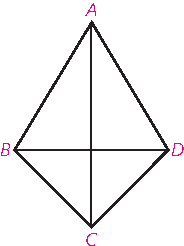
\includegraphics[scale=1.2]{"Shapes/Fasl - 3/Dars 2/P72-S1.pdf"}
	\captionof{figure}{تمرین ۱}
\end{Figure}

\bigskip

{\medium ۲-} در چهارضلعی
\lr{ABCD}،
مطابق شکل 
$AB = AD$
و
$BC = CD$
است. آیا قطرهای این چهارضلعی برهم عموداند؟ چرا؟ نشان دهید در این چهارضلعی قطر 
$AC$
روی نیمسازهای
$\angle A$
و
$\angle C$
است. اگر اندازه های دو قطر ۸ و ۶ باشند، مساحت آن را محاسبه کنید. چهارضلعی ای با این ویژگی کایت نام دارد. نشان دهید در کایت یک قطر عمودمنصف قطر دیگر است.
\bigskip

{\medium ۳-}
در شکل دو خط d و d' موازی‌اند و ABCD و ABEF هردو متوازی الاضلاع اند. اگر مساحت یکی از این متوازی الاضلاع ها برابر S باشد، مساحت دیگری برحسب S چقدر است؟

\begin{Figure}
	\centering
	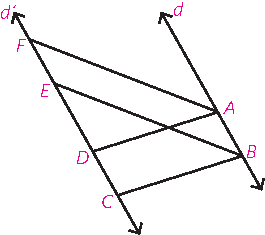
\includegraphics[scale=1.2]{"Shapes/Fasl - 3/Dars 2/P72-S2.pdf"}
	\captionof{figure}{تمرین ۳}
\end{Figure}

\bigskip
{\medium ۴-}
در ذوزنقهٔ شکل مقابل اندازه های دو قاعده a و b و اندازه های دو زاویهٔ مجاور به یک قاعده 
$^{\circ}$45
 است. مساحت ذوزنقه را برحسب a و b محاسبه کنید. از A و B بر قاعده DC عمود کنید.

\begin{Figure}
	\centering
	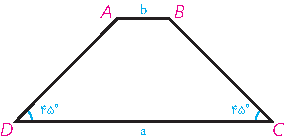
\includegraphics[scale=1.2]{"Shapes/Fasl - 3/Dars 2/P72-S3.pdf"}
	\captionof{figure}{تمرین ۴}
\end{Figure}


\bigskip
{\medium ۵-}
مساحت ذوزنقهٔ مقابل را به دو طریق به دست آورید. از مساوی قرار دادن آنها چه نتیجه ای به دست می‌آید؟

\begin{Figure}
	\centering
	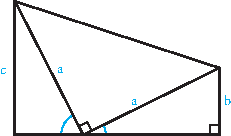
\includegraphics[scale=1.2]{"Shapes/Fasl - 3/Dars 2/P72-S4.pdf"}
	\captionof{figure}{تمرین ۵}
\end{Figure}


\bigskip
{\medium ۶-}
در متوازی الاضلاع ABCD، M وسط ضلع BC است و پاره خط AM قطر BD را در N قطع کرده است. نشان دهید: \hfill
	$
\mathrm{S}_{\mathrm{BMN}} = \dfrac{1}{12} \mathrm{S}_{\mathrm{ABCD}}
	$


\begin{Figure}
	\centering
	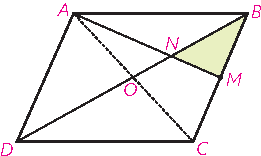
\includegraphics[scale=1.2]{"Shapes/Fasl - 3/Dars 2/P72-S5.pdf"}
	\captionof{figure}{تمرین 6}
\end{Figure}


{\medium ۷-}
در مثلث ABC، خط MN موازی ضلع BC است و 
$ \dfrac{AM}{MB} = \dfrac{1}{2} $.
همچنین 
$ \dfrac{PC}{PB} = \dfrac{1}{3} $
است. 
$ \mathrm{S}_{\mathrm{AQN}} $ و $\mathrm{S}_{\mathrm{MQPB}}$
چه کسری از مساحت مثلث ABC است؟

\begin{Figure}
	\centering
	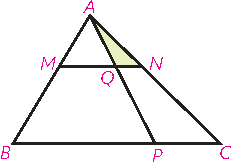
\includegraphics[scale=1.2]{"Shapes/Fasl - 3/Dars 2/P73-S1.pdf"}
	\captionof{figure}{تمرین 7}
\end{Figure}

\bigskip
{\medium ۸-}
با توجه به مساحت چند ضلعی‌های شبکه‌ای
 (شکل \ref{fig:p73-s2})،
  مساحت قسمت سایه زده را محاسبه کنید.
{{\small (راهنمایی: مساحت چند ضلعی داخلی را از مساحت چند ضلعی بیرونی کم کنید.)}

\begin{Figure}
	\centering
	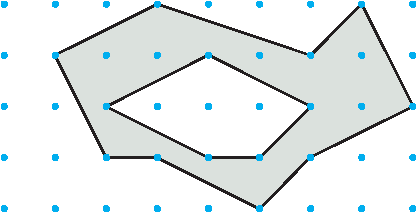
\includegraphics[width=0.9\linewidth]{"Shapes/Fasl - 3/Dars 2/P73-S2.pdf"}
	\captionof{figure}{تمرین 8}
	\label{fig:p73-s2}
\end{Figure}

\bigskip
{\medium ۹-}
یک مستطیل شبکه ای با ضل عهای افقی و قائم که اندازه های ضلع‌های آن m و n واحداند مفروض است. مساحت آن را ابتدا به روش معمول و سپس به کمک فرمول پیک محاسبه و آنها را مقایسه کنید.

\bigskip
{\medium ۱۰-}
مساحت یک چند ضلعی شبکه‌ای ۳ واحد است. جدولی تشکیل دهید و تعداد نقاط مرزی و تعداد نقاط درونی را در حال تهایی که امکان دارد، مشخص کنید. اگر این چندضلعی شبک های مثلث باشد در هر حالت شکل آن را رسم کنید. در حالتی که نقاط مرزی بیشترین تعداد ممکن را دارند، شکل‌های چهارضلعی‌های نظیر آن را نیز رسم کنید.

}\end{multicols}

\newpage

\subsection{پاسخ}
\chapter{تجسم فضایی}

\section{خط، نقطه و صفحه}

\section{تفکر تجسمی}

	
\end{document}